\documentclass[a4paper,11pt,uplatex]{jsbook}

%\usepackage{fancyhdr}
\setlength{\footskip}{16pt}
\usepackage{amsmath}
\usepackage[dvipdfmx]{graphicx}
\usepackage[dvipdfmx]{color}
%\usepackage{pagecolor}[white]
\usepackage{amsmath,amssymb}
%\usepackage[top=3cm, bottom=3cm, left=3cm, right=3cm]{geometry}
\usepackage{braket}
\usepackage{bm}
\numberwithin{equation}{section}
\usepackage{mathrsfs}
\usepackage{siunitx}
\usepackage{physics}
\usepackage[dvipdfmx]{graphicx}
\usepackage[compat=1.1.0]{tikz-feynhand}
\usepackage{caption}
\usepackage{subcaption}
%\usepackage{cleveref}
\usepackage{float}
\usepackage{multicol}
\setlength{\columnsep}{15mm}
%\usepackage[style=phys,articletitle=false,biblabel=brackets,chaptertitle=false,pageranges=false]{biblatex}
%\usepackage[style=phys]{biblatex}
\usepackage[dvipdfmx]{hyperref}
\usepackage{url}
\usepackage{pxjahyper}
\usepackage{bookmark}
%\usepackage[backref]{hyperref}
\setcounter{tocdepth}{3}
\setlength{\parindent}{2em}
\def\vector#1{\mbox{\boldmath $#1$}}
\def\slash#1{\not\!#1}
\def\slashb#1{\not\!\!#1}
\def\delsla{\not\!\partial}
%\usepackage[dvipdfmx]{xcolor}


\hypersetup{
 setpagesize=false,
 bookmarksnumbered=true,%
 bookmarksopen=true,%
 colorlinks=true,%
 linkcolor=black,
 citecolor=red,
 urlcolor=black,
}
%backreferenceのカスタマイズ. "Back to p.3"のように表示する.
%\renewcommand*{\backref}[1]{(p.#1へ戻る)}
%\newcommand{\backtoc}{\hyperlink{toc}{[目次へ]}}
\newcommand{\backtoc}{\texorpdfstring{\protect\hyperlink{toc}{\hspace{5pt} \scriptsize [目次へ]}}{}}
\newcommand{\mychapter}[1]{\chapter[#1]{#1\backtoc}}
\newcommand{\mysection}[1]{\section[#1]{#1\backtoc}}
\newcommand{\mysubsection}[1]{\subsection[#1]{#1\backtoc}}
% 数式
%\usepackage{amsmath,amsfonts}
%\usepackage{bm}
%\usepackage{physics}
%\usepackage{siunitx}
% 画像
%\usepackage[dvipdfmx]{graphicx}
%\usepackage[dvipdfmx,colorlinks=true,linkcolor=blue]{hyperref}
%\usepackage{pxjahyper}

\begin{document}

\chapter{導入}
\section{ハイパー核}
本論文は、ドイツ、マインツ大学にある連続電子線加速器マインツマイクロトロン(MAMI)における200 MeV領域の電子ビームエネルギー測定について論じる。
電子ビームエネルギーの絶対値を$\delta \text{E}/\text{E} \sim 10^{-4}$の精度で測定し、磁気運動量スペクトロメータの系統誤差を$\delta p/p \sim 10^{-4}$に抑えることで、
過去に我々が測定した$^4_{\Lambda} \text{H}$における$\Lambda$粒子の束縛エネルギーの精度$100$ keVから向上させ、
ハイパートライトン$^3_{\Lambda}\text{H}$における$\Lambda$束縛エネルギーを10 keVを切る精度で決定することを目指す。
ハイパートライトンにおける$\Lambda$束縛エネルギーの決定精度向上は、まだ謎の多い$\Lambda$N相互作用に対しさらなる知見を与える。

本章でははじめにハイパー核とその研究の歴史、ハイパー核生成実験について述べる。次に我々がマインツマイクロトロンにおいて独自に開発した$\Lambda$ハイパー核精密質量分光手法である
崩壊パイ中間子法とその課題となっている電子ビームエネルギー測定精度の重要性について述べた後、最後に本研究の目的を述べる。

\subsection{ハイペロンとハイパー核}
素粒子の標準理論によれば、自然界の粒子は全てそれ以上分割できない最小単位の粒子(素粒子)からなり、素粒子の間に働く力は、強い力、弱い力、電磁気力、重力の4種類の力であると理解されている。
素粒子は物質を構成する粒子と力を媒介する粒子に分類でき、さらに物質を構成する粒子は強い相互作用をするクォークと強い相互作用をしないレプトンに分類できる。
クォークは表\ref{tab:quark}に示すように三世代に分類されている。
\begin{table}[ht]
\centering
\begin{tabular}{|c||c|c|c||c|c|}
  \hline
  & 1世代 & 2世代 & 3世代 & 電荷 & スピン\\
  \hline\hline
  クォーク & u & c & t & $+2/3$e & 1/2\\
  & d & s & b & $-1/3e$ & 1/2\\ \hline
  レプトン & e& $\mu$& $\tau$& $-e$& 1/2\\
  &$\nu_e$ & $\nu_\mu$& $\nu_\tau$& 0 & 1/2\\
  \hline
\end{tabular}\label{tab:quark}
\caption{クォークとレプトンの一覧}
\end{table}

クォークは単体で存在することはできず、一般に3つ集まったバリオンか2つ集まったメソンの形で存在する。我々の身の回りの物質はハドロンである陽子と中性子からなる原子核と、その周りを囲む電子からなる原子によって構成されている。
陽子、中性子は特に通常原子核を構成する意味で核子(nucleon)と呼ばれている。

構成子クォークモデルでは、陽子はuudクォーク、中性子はuddクォークからなり、それぞれ電荷+1と0を持つ。クォークにはそれぞれアイソスピンと呼ばれる量子数を導入することでスピン演算子と同じ枠組みで扱うことができることが知られている。
%荷電対称性 pp nn核力はほぼ等しい
uクォーク、dクォークはそれぞれアイソスピン+1/2、$-$1/2を持ち、陽子、中性子は+1/2、$-$1/2を持つ。強い相互作用はアイソスピンのSU(2)空間回転に対してほとんど対称であることが知られている。
u、dクォークのSU(2)対称性にsクォークを加えて拡張したSU(3)対称性は、u、dクォークに比べてsクォークが比較的重く、疑似的な対称性とみなされている。
これらu、d、sクォークからなるバリオンはフレーバーSU(3)の枠組みにおいて、スピン1/2のバリオン8重項、スピン3/2のバリオン10重項に分類される(図\ref{fig:baryon})。
%heavy だともっと重くて、対称性が破れるという話も入れるとよい
\begin{figure}[tb]
  \centering
  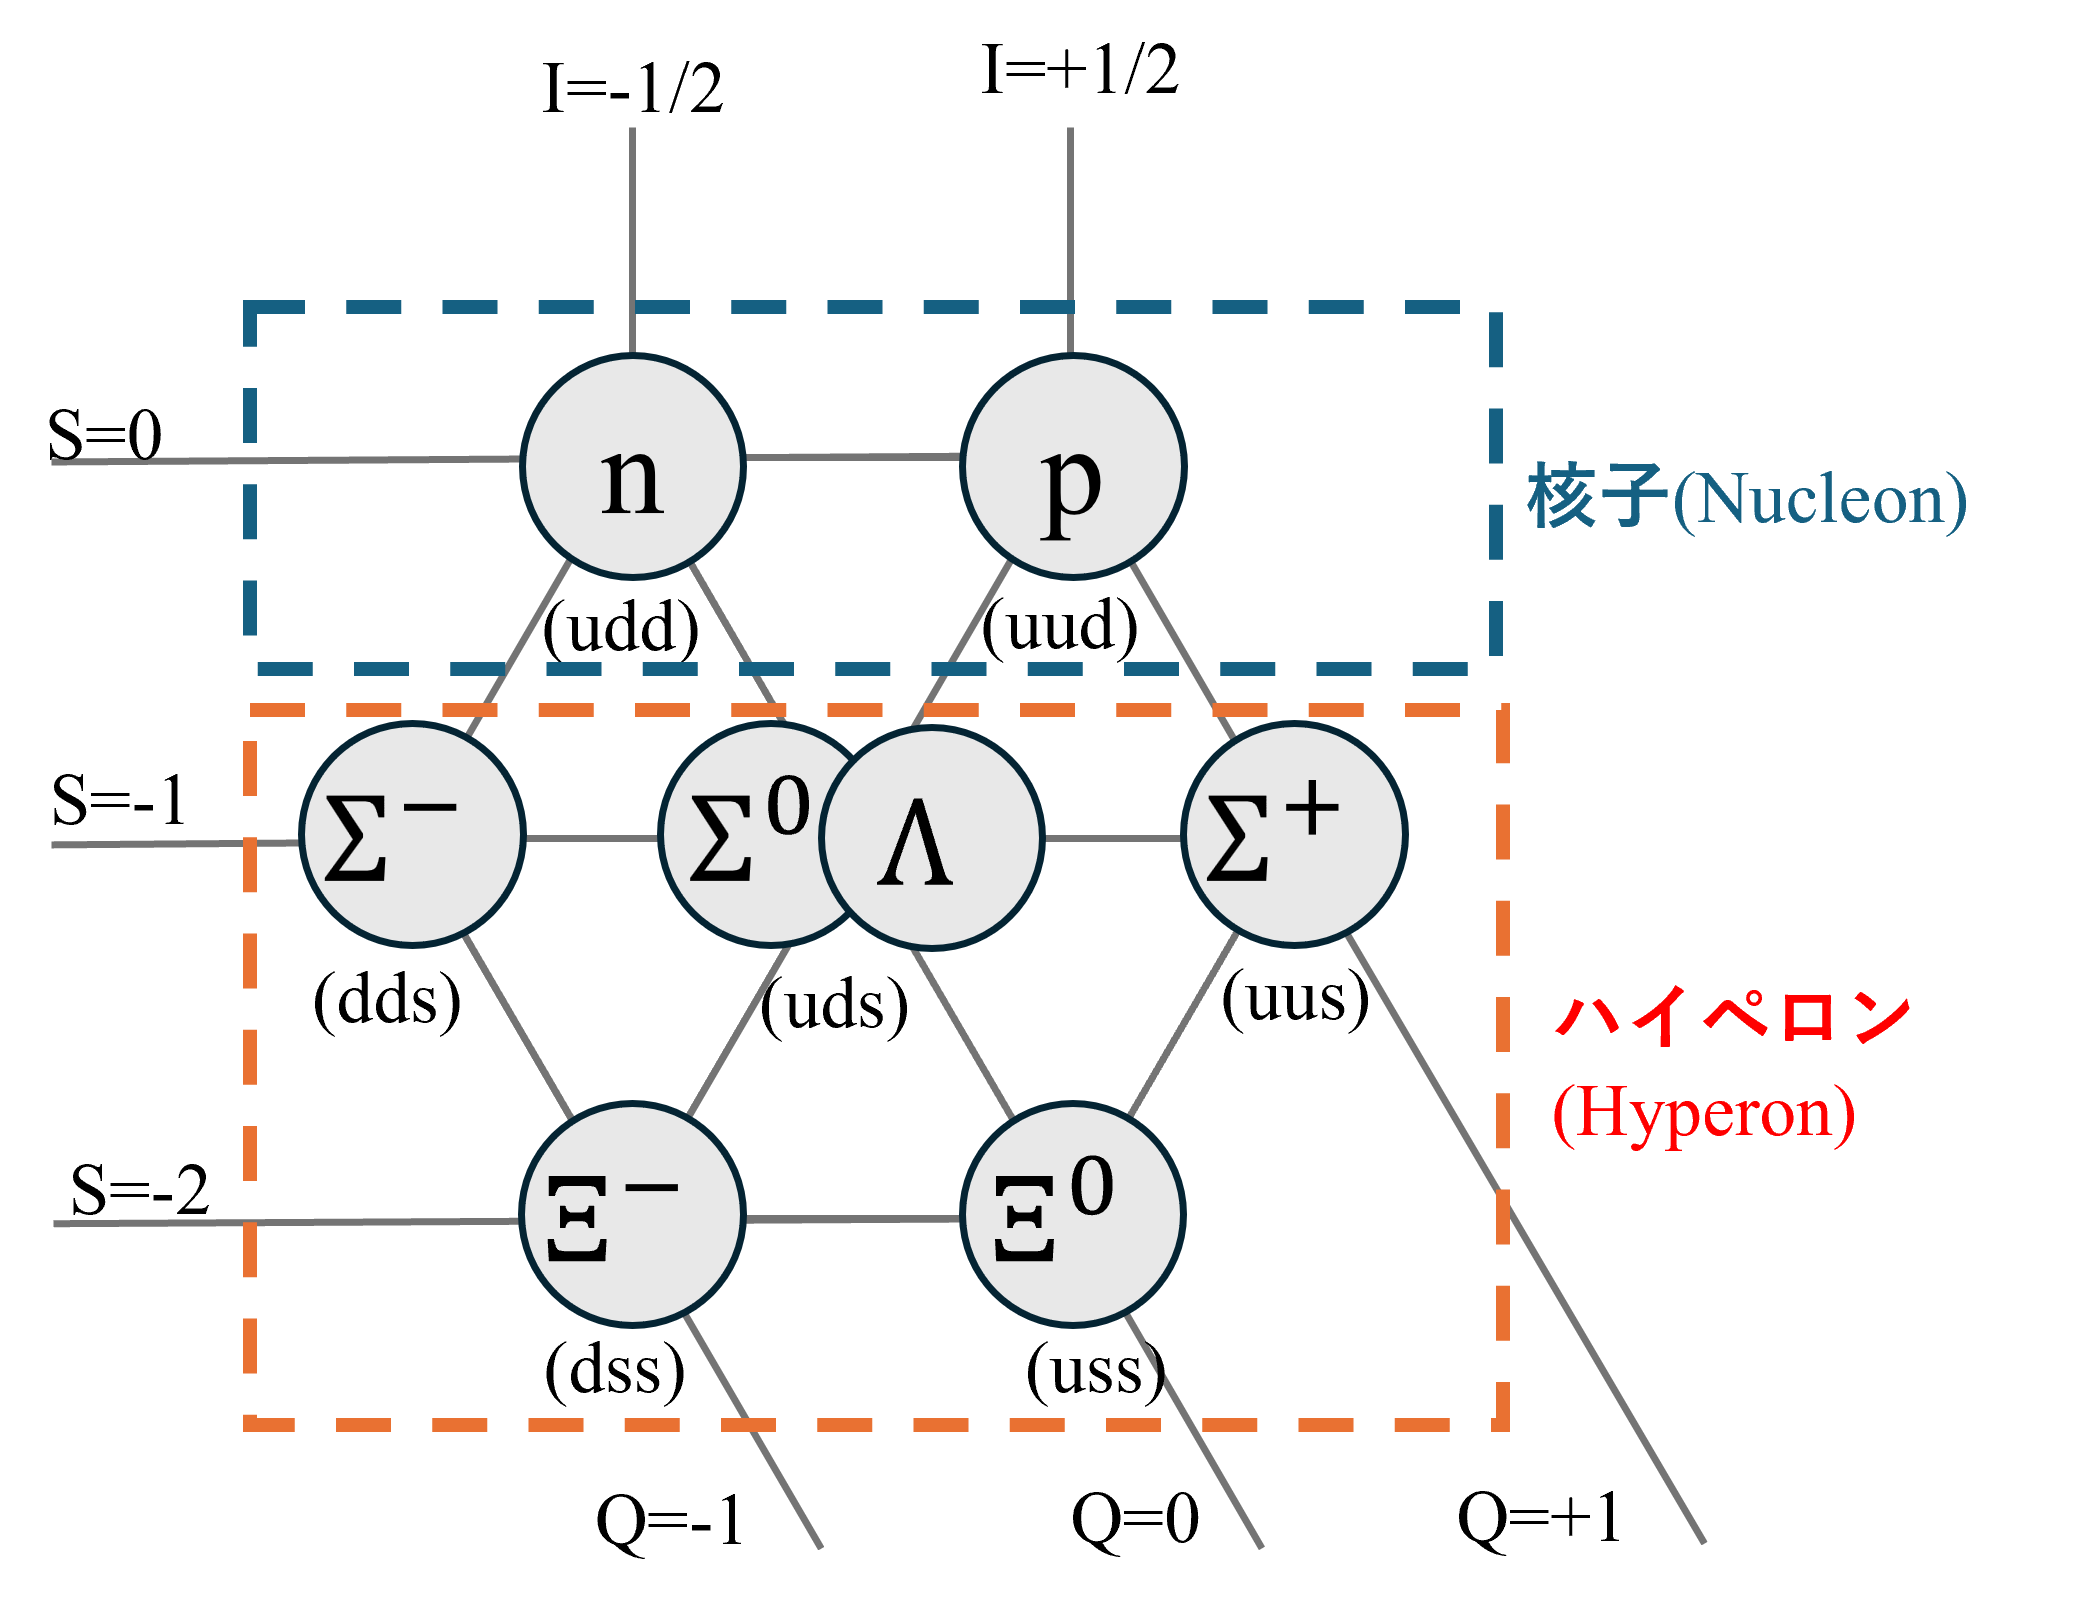
\includegraphics[width=10cm]{image/1_baryon.png}
  \caption[バリオン8重項]{バリオン8重項。アイソスピンI、電荷Qに加え、ストレンジネスSの計3つの量子数を示した}
  \label{fig:baryon}
\end{figure}


特にsクォークを含むバリオンをハイペロンと呼ぶ。その中でもu、d、sクォークからなるΛ粒子は最も軽い基本的なハイペロンである。
\begin{table}[h]
\centering
\begin{tabular}{|c|c|c|c|c|}
  \hline
  ハイペロン&質量(MeV/$c^2$)&寿命 (s)&主な崩壊モード&分岐比(\%)\\
  \hline \hline 
  \multirow{2}{*}{$\Lambda$} & \multirow{2}{*}{1115.683(6)} & \multirow{2}{*}{$2.632(10) \times 10^{-10}$} & $p + \pi^-$ &63.9\%\\
                             &                              &                                              & $n + \pi^0$ & 35.8\\ \hline
  $\Sigma^0$                 & 1192.642(4)                  & $7.4(7) \times 10^{-20}$                     & $\Lambda + \gamma$ & 100\\ \hline
  \multirow{2}{*}{$\Sigma^+$}& \multirow{2}{*}{1189.37(7)}  & \multirow{2}{*}{$0.799(5) \times 10^{-10}$}  & $p + \pi^0$ & 51.6\\
                             &                              &                                              & $n + \pi^+$ & 48.5\\ \hline
  $\Sigma^-$                 & 1197.45(7)                   & $0.486(5) \times 10^{-10}$                   & $n + \pi^-$ & 99.9\\ \hline
\end{tabular}
\caption{ハイペロンの性質}
\end{table}

原子核中に核子だけでなくハイペロンを含む原子核をハイパー核と呼ぶ。ハイパー核には通常核子には見られない性質が現れることが知られており、それ自体が重要な研究対象である。
ここではハイパー核の性質の一つとして、崩壊モードについてこの章で詳しく述べる。
%λΣの表の説明を本文にも入れる
自由空間ではΛ粒子の寿命は$10^{-10}$秒程度で、$\pi$中間子を放出して崩壊する。これは中間子弱崩壊と呼ばれる。

一方Λ粒子が原子核に束縛されているハイパー核の場合には、中間子弱崩壊で$\pi$中間子とともに放出された核子が、原子核の他の核子の影響を受けてフェルミの排他律を受けることにより、中間子弱崩壊が抑制される。
その結果、中間子を放出しないような崩壊、いわゆる非中間子弱崩壊が主な崩壊モードとなる。

軽いハイパー核の場合には核子によって占められているフェルミ準位が低いため、重いハイパー核と比較すると中間子弱崩壊が起こりやすいと言える。

\subsection{ハイパー核研究の意義}
ハイパー核研究において、通常核子間の核力(NN相互作用)に加えてハイペロンと核子の相互作用(YN相互作用)を調べることができる。
ハイパー核の研究では、このYN相互作用の知見を得ることが一つの重要なモチベーションとなっている。

YN相互作用に関する重要な研究テーマにはハイペロンパズル、荷電対称性の破れ、ハイパートライトンパズル等がある。
\subsubsection{ハイペロンパズル}
中性子星内部では、中性子のフェルミエネルギーがΛ粒子の生成エネルギーを上回るため、$\Lambda$粒子が生成されると考えられる。したがって中性子星内部の状態方程式には$\Lambda$N相互作用の項が自然に含まれると考えられる。
現在のΛN相互作用の理解に基づく状態方程式によると、中性子星の質量は太陽質量の2倍よりも大きくなることはないとされている。
しかし近年、宇宙観測によって太陽質量の2倍以上の質量をもつ中性子星が観測されており、この矛盾がハイペロンパズルとして注目されている。
%citationする
ハイペロンパズルの解決には$\Lambda$N相互作用のより正確な知見が不可欠である。
\subsubsection{荷電対称性の破れ}
NN相互作用においては、クーロン力の効果を除いた核力は荷電対称性を持つ。すなわち、陽子と中性子は核力においてほとんど区別されない。特に質量数A=3程度の軽い原子核において、実験と理論の両側面から荷電対称性の破れは数keV程度の精度で理解されている。

一方でΛ粒子と核子間の相互作用には荷電対称性の破れが存在することが示唆されており、$\Lambda$N相互作用の更なる理解が求められている。
%もっと詳しく。この背景があって4LHがあるんだ、という話
\subsubsection{ハイパートライトンパズル}
\ref{sec:hypertriton puzzle}章で詳しく述べる。
\subsubsection{NN相互作用}
YN相互作用の理解だけでなく、ハイペロンが原子核深部のプローブとしてNN相互作用の解明にも役立つ。ハイペロンは核子と異なる粒子であるためパウリの排他律を受けず、深い軌道にも束縛される。
この性質を利用して核子を用いた反応では調べることのできない核子間相互作用を調べることができる。%原子核の深部のプローブとして役に立つ
%原子核の深部にバリオンの振る舞いを見たい、ラムダをいれて構造を変えてみる。
\subsection{ハイパー核質量分光}
ハイパー核を生成し、その質量を測定する実験手法を質量分光と呼ぶ。ハイパー核の生成反応は主に$(K^-, \pi^-)$反応、$(\pi^+, K^+)$反応、$(e,e'K^+)$反応がある。

\begin{figure}[b]
  \centering
  \begin{subfigure}[b]{0.47\linewidth}
    \centering
    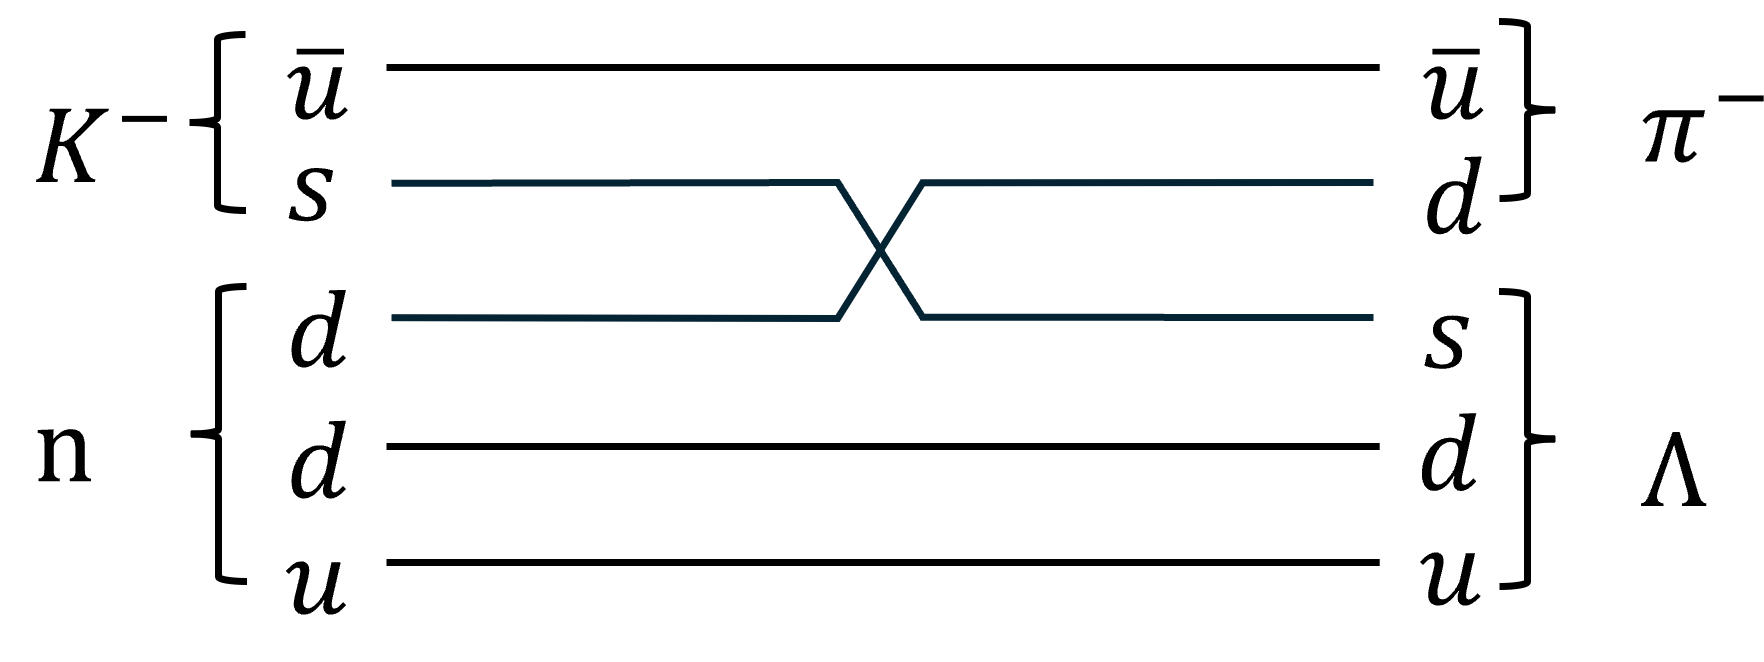
\includegraphics[width=\linewidth]{image/1-Kpi.png}
    \subcaption{($K^-, \pi^-$)反応}
  \end{subfigure}
  \hfill
  \begin{subfigure}[b]{0.47\linewidth}
    \centering
    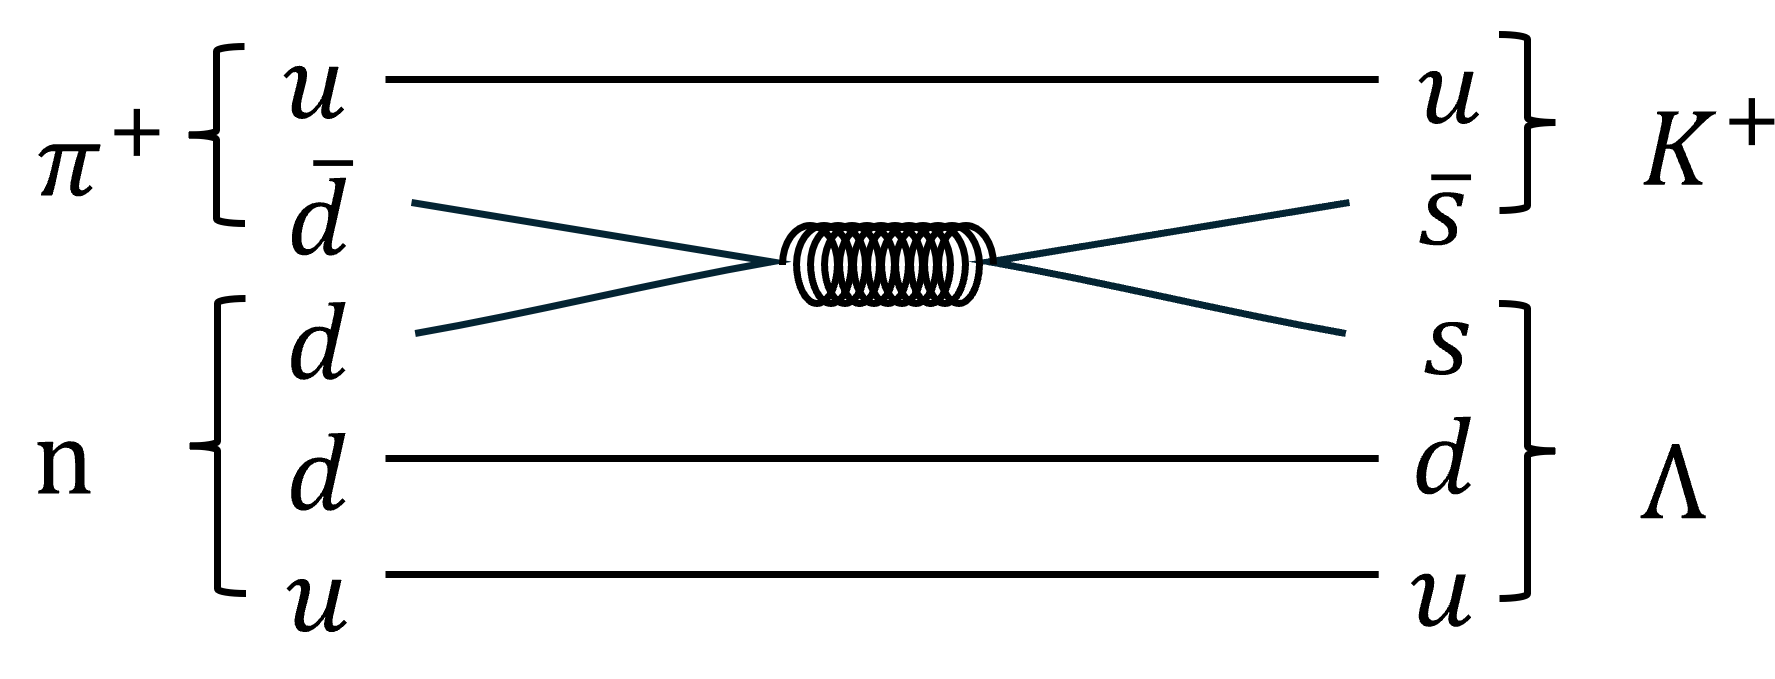
\includegraphics[width=\linewidth]{image/1-piK.png}
    \subcaption{($\pi^+, K^+$)反応}
  \end{subfigure}
  \begin{subfigure}[b]{0.5\linewidth}
    \centering
    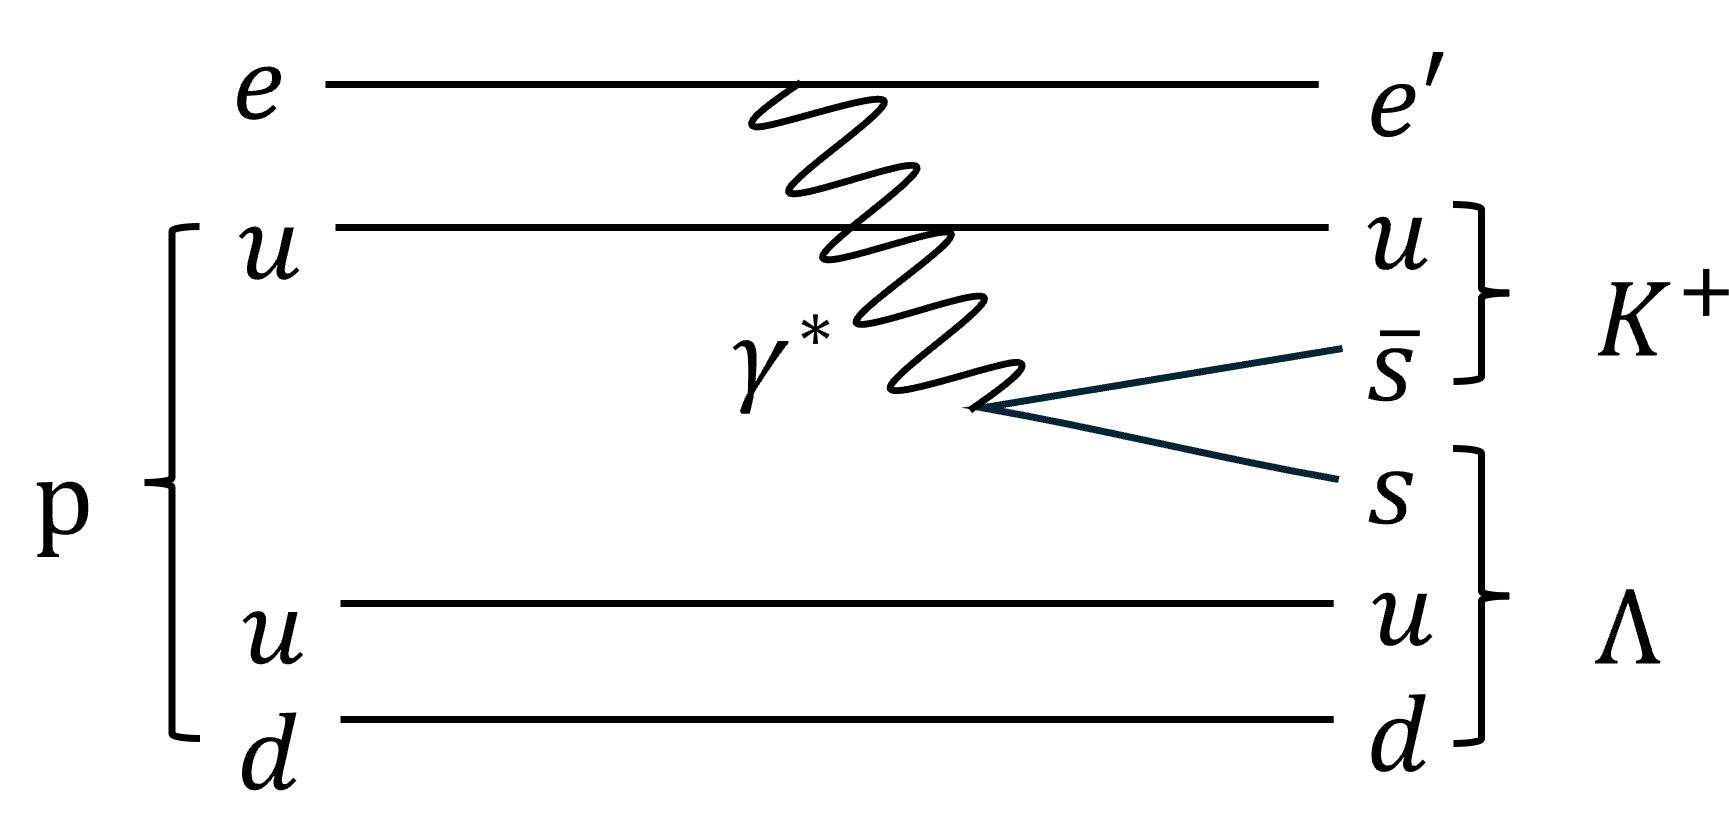
\includegraphics[width=\linewidth]{image/1-eeK.png}
    \subcaption{($e,e'K^+$)反応}
  \end{subfigure}
  \caption[主なハイパー核生成反応のファインマンダイアグラム]{}
\end{figure}

\subsubsection{($\text{K}^-, \pi^-$)}
クォーク交換反応である。sクォークを生成する必要がないため、Λ粒子の生成断面積が mb/srと大きい。
\subsubsection{($\pi^+, \text{K}^+$)}
核内で$\text{d}$,$\bar{\text{d}}$クォークが対消滅し、$\text{s}$,$\bar{\text{s}}$クォークが生成される。この反応はΛ粒子の生成断面積が100 $\mu$b/srと小さいが、
一般にKビームよりも$\pi^-$ビームが強度の高いビームを得られるため、問題とならない。
運動量移行が大きいため、$\Lambda$が様々な軌道角運動量に入った状態を生成することができる。
\subsubsection{$(e,e'K^+)$}
電子ビームを用いて、仮想光子を媒介して$\text{s}$,$\bar{\text{s}}$クォークを生成する反応である。電磁相互作用による反応であり、生成断面積は100 nb/srと小さいが、
電子ビームは高い強度が得られるため、十分な統計量を得ることができる。更に$\pi$,Kといった中間子ビームは二次ビームであるのに対して、
加速器で直接加速した高品質な一次電子ビームを用いることができるため、高い分解能を得ることができる。
%ハイパー核の生成反応か、素過程の反応かで話が変わってきそうだから一応確認


生成したハイパー核の質量は、入射ビーム運動量及び崩壊によって生成する粒子の運動量、エネルギーを測定することで、欠損質量法や不変質量法によって求めることができる。
%欠損質量、不変質量法の説明を注釈的に
\subsubsection{原子核乾板実験}
%原子核乾板の説明が必要
原子核乾板中を荷電粒子が通過すると、乾板中の原子核が電離される。電離電子によって乾板中の銀イオンが結合し、粒子の軌跡が残る。
この軌跡を読み取ることで、粒子の識別、運動量測定を同時に行うのが原子核乾板による粒子検出法、質量分光法である。
\subsubsection{重イオン衝突実験}
原子核同士を衝突させると様々な反応が同時に起こる。これを利用してハイパー核を生成し、生成した粒子の運動量の相関からハイパー核の質量を測定することができる。
%invariant massを組む。相関はfemtoscopyなので訂正が必要
\subsection{ハイパートライトンパズル}\label{sec:hypertriton puzzle}
ハイパー核の中でも最も基本的な束縛系が$^3_{\Lambda}\text{H}$、ハイパートライトンである。これは陽子、中性子、Λ粒子がそれぞれ一つずつからなるハイパー核である。
1960年代に原子核乾板や泡箱実験によって$B_{\Lambda} = 130 \pm 50(\text{stat.}) \pm 40(\text{syst.})$ keVとされており、この結果が約50 年間信じられてきた。
%citation入れる
100 keV程度の弱い束縛から、%口語的な表現を避ける
Λ粒子は陽子、中性子に対してハロー構造のような状態であると示唆される。%もう少し説明を加える、波動関数の半径が鉛くらい、の論文、だからほぼ自由空間のΛ粒子と同じ状態
従ってその寿命は自由空間のΛ粒子と同程度であると見積もられる。\\
これに対して2010年台に重イオン衝突実験が、ハイパートライトンの寿命が予測よりも有意に短いことを示唆する実験結果を次々と報告した。これらの値は$\tau \sim$200 psであり、
$B_{\Lambda} = 130$ keVの結果と整合性のある物理的な解釈はいまだない。この問題をハイパートライトンパズルと呼ぶ。\\
2020 年代にSTAR,ALICEの2つの重イオン衝突実験が報告した結果によれば、それぞれ$B_{\Lambda}= 102 \pm 63(stat.) \pm 67(syst.)$ keV, 
$B_{\Lambda} = 406 \pm 120(stat.) \pm 110 (syst.)$ keVであり、どちらのグループの結果も系統誤差が比較的大きい。\\
%citation入れる。視覚的にもわかりやすいように図を入れる

%反応分光法に(pi K)があり、それとならんでDPS、重イオン、原子核乾板があるという書き方をする
\section{崩壊パイ中間子法}
崩壊パイ中間子法は2010年代にドイツのマインツ大学マイクロトロン(MAMI)で我々の研究グループによって開発されたハイパー核の質量分光法である\cite{esserObservation4Hyperhydrogen2015}。
10 keVを切る高いエネルギー分解能が実証されている\cite{Schulz2015} ため、ハイパートライトンパズルの解明に有効な手法であると期待されている。
この章では崩壊パイ中間子法の原理を述べる(\ref{sec:dps principle}節)。そして高い分解能が実現できる理由と、解決すべき課題について述べる。
\subsection{原理}\label{sec:dps principle}
電子ビームで電磁生成したハイパー核が核破砕し、目的のハイパー核が標的中で静止し2体崩壊する反応を検出する。
この時ハイパー核の質量$m(^A_{\Lambda}Z)$は2体崩壊に注意すると
\begin{eqnarray}
  m(^A_{\Lambda}Z) = \sqrt{m(^A(Z+1))^2 + p^2_\pi} + \sqrt{m_\pi^2 + p_\pi^2} \label{mass formula}
\end{eqnarray}
%c=1にしていることを注釈でいれる
と$\pi$中間子の運動量$p_\pi$のみで求めることができる。

Λハイパー核の質量$m(^A_\Lambda Z)$からこのハイパー核における$\Lambda$粒子の束縛エネルギー$B_\Lambda$は、$\Lambda$粒子を除いたコア核の質量$m_{core}$と$\Lambda$粒子の質量$m_\Lambda$を用いて
\begin{eqnarray}
  B_\Lambda = m_{core} + m_\Lambda - m(^A_\Lambda Z) \label{binding energy formula}
\end{eqnarray}
と求めることができる。
\\ハイパートライトンがパイ中間子を放出する崩壊モードは
\begin{eqnarray}
  ^3_{\Lambda}\text{H} \rightarrow ^3\text{He} + \pi^-
\end{eqnarray}
であるから、式(\ref{mass formula})、式(\ref{binding energy formula})より、$m(^3_\Lambda\text{H})$
\begin{eqnarray}
  m(^3_\Lambda \text{H}) &= \sqrt{m(^3\text{He})^2 + p^2_\pi} + \sqrt{m_\pi^2 + p_\pi^2} \\
  B_\Lambda &= m_{^2\text{H}} + m_\Lambda - m(^3_\Lambda \text{H})
\end{eqnarray}
とかける。$p_\pi$を除く$m(^3\text{He})$、$m_\pi$、$^2\text{H}$は高精度で求まっているため、
%高精度の定量的に
$B_\Lambda$の決定精度は、静止かつ2体崩壊という崩壊の特徴により放出される単色$p_\pi$の不確かさによって決まる。
さらに、パイオンの運動量は単色的である。従って$p_\pi$の不確かさは$p_\pi$の分解能によってのみ決められる。
これが崩壊パイ中間子法が高い質量分解能を実現できる理由である。
%いいスペクトロメータがあればという話でもよいかも
%Kタグの話もここで入れる。

\subsubsection{マインツマイクロトロン(MAMI)}
我々の研究グループはドイツ、マインツ大学マイクロトロン(MAMI)において、崩壊パイ中間子法を用いてハイパー核の質量分光を行ってきた。
質量分光実験を行う実験ホール(A1 Hall)には、標的チェンバーを中心に、磁気運動量スペクトロメータ(Spek A,C)、Kaosスペクトロメータが配置されている。
\begin{figure}[tb]
  \centering
  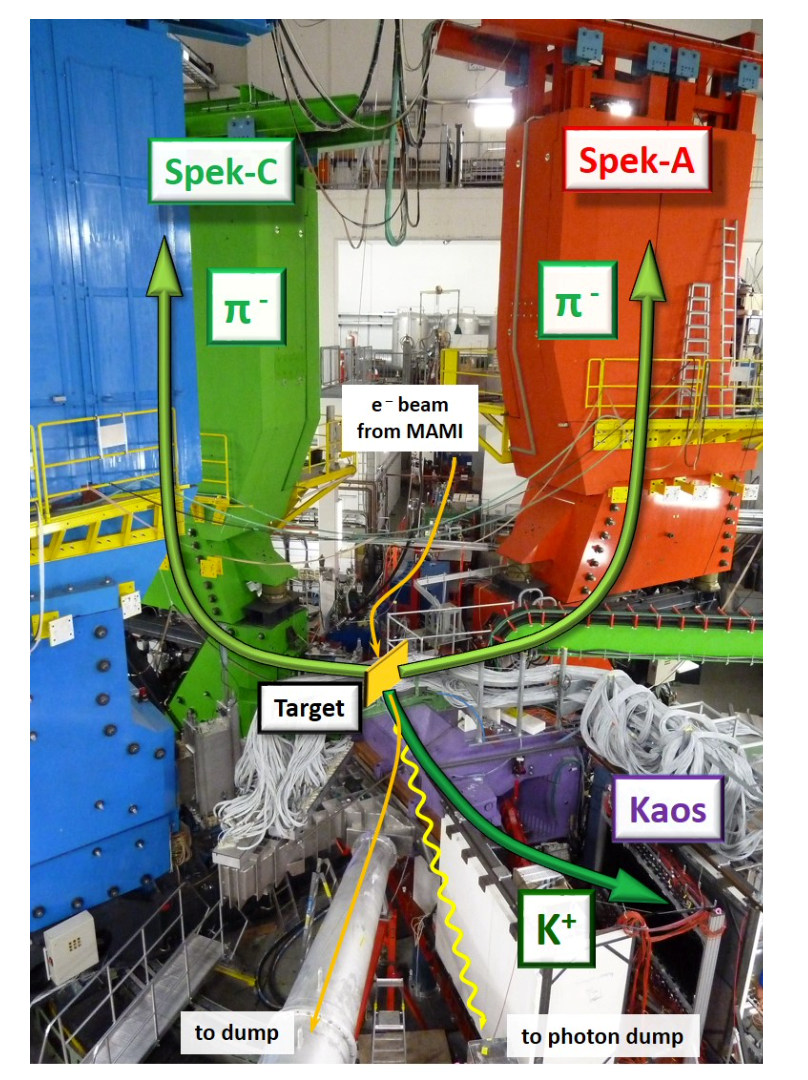
\includegraphics[width=10cm]{image/1-HallA.png}
  \caption[MAMI実験ホール]{A1 Hall概観図。MAMI加速器で加速された電子がビームラインを通って標的チェンバー内の標的に照射される。崩壊パイ中間子法では、照射されて生成されたハイパー核が崩壊する際の$\pi$中間子の運動量を
  Spek A,Cで測定する。またKaosスペクトロメータでは$K^+$中間子の粒子識別を行うことでイベント選択を行う。}
\end{figure}

2014年に行った$^4_{\Lambda}\text{H}$の実験\cite{Schulz2015}では、$\pi$中間子の運動量が
$p_\pi = 132.867 \pm 0.007(\text{stat.}) \pm 0.106(\text{syst.})$ MeV/$c$と測定され、10 keV以下の運動量分解能を実現している。
\begin{figure}[b]
  \centering
  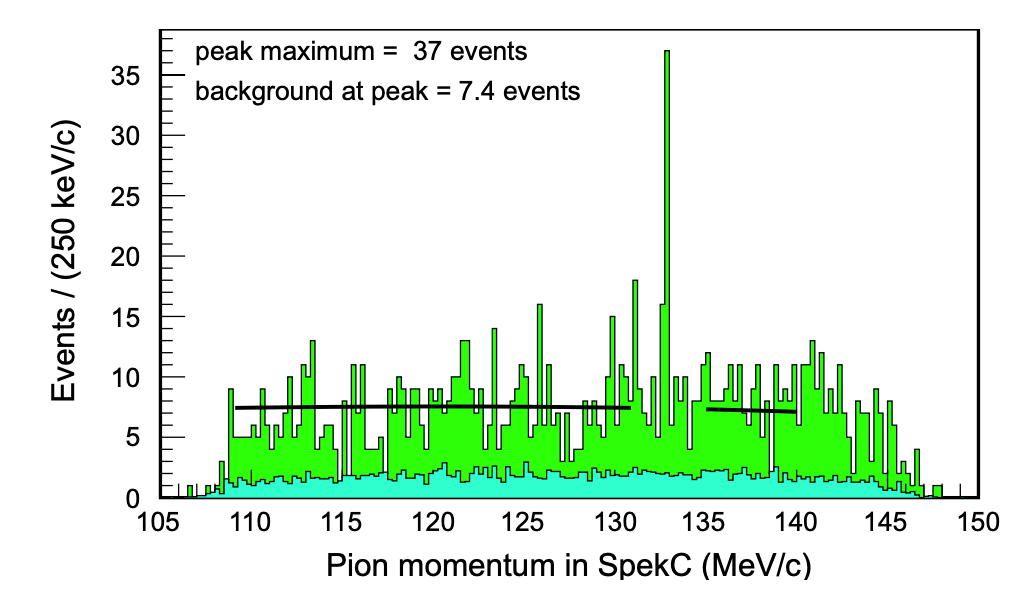
\includegraphics[width=10cm]{image/1-PionSpectrum.png}
  \caption[過去実験での$p_\pi$スペクトル]{高分解能の$\pi$中間子スペクトル。細いピークが133 MeV/c付近に位置しており、これは$^4_{\Lambda}\text{H}$の崩壊で得られる$p_\pi$である\cite{Schulz2015}}
\end{figure}
%図の引用をする

ここから、$^4_{\Lambda}\text{H}$の$\Lambda$粒子の束縛エネルギー$B_\Lambda$は$B_\Lambda = 2.157 \pm 0.005(\text{stat.}) \pm 0.077(\text{syst.})$ MeVと決定された。

MAMIの持つ高分解能運動量スペクトロメータ(Spek A,C)によって実現される高い分解能は、他のハイパー核質量分光法や重イオン衝突実験では実現できない。
これは崩壊パイ中間子法の大きな特徴であると言える。
ただし、崩壊パイ中間子法は基底状態にのみ適用できるという点で他の手法とは相補的である。

\subsubsection{磁気運動量スペクトロメータ(Spek A, Spek C)}
ハイパー核の崩壊に伴う$\pi$中間子の運動量$p_\pi$を測定するためには、MAMIの磁気運動量スペクトロメータを用いる。
実験ホール内のスペクトロメータはSpek A,Cの2つのスペクトロメータと後段のKaosスペクトロメータから構成される。Spek A,Cでは$\pi$中間子の運動量を精密に測定するのに対し、Kaosでは$K^+$を検出することでΛハイパー核が生成されたイベントの選択に用いる。
%Kaosは
運動量測定用のSpek A,C は電磁石と飛跡検出用のドリフトチェンバー、粒子識別用のシンチレーションカウンターとチェレンコフ光検出器から構成されている。
入射した荷電粒子は電磁石によって曲げられるが、その曲率は粒子の運動量に依存する。この性質を利用することで、ドリフトチェンバーによる位置測定の結果から入射粒子の運動量を決定することができる。


\subsection{系統誤差}
10 keVを切る束縛エネルギーの統計誤差に対して、崩壊パイ中間子法の系統誤差は100 keV程度と大きい。
これは$p_\pi$の決定精度に対する系統誤差が100 keV程度あることに由来する。
磁気スペクトロメータの運動量絶対値較正のためにMAMIでは電子弾性散乱を利用している。
標的の質量を$m_T$、電子質量を$m_e$、入射電子ビームのエネルギーを$E_{beam}$として、標的で弾性散乱された電子の運動量$p_e'$は散乱角$\theta$に対して一意に決まり、
\begin{eqnarray}
  p_e' = \sqrt{\left(\frac{E_{beam}}{1 + E_{beam}/m_T(1 - \cos{\theta})} \right)^2 - m_e^2}\label{elastic scattering}
\end{eqnarray}
と計算できる。散乱角と入射エネルギーに対して弾性散乱のピークから運動量の絶対値を較正する。
ハイパー核の崩壊で放出される$\pi$の運動量はおよそ 100 - 140 MeV/c の領域にあるため、散乱電子も同程度の運動量であることが望ましい。
MAMIの電子線加速器が出せる最低エネルギーである180、195、210 MeVの3種類のエネルギーに対して電子弾性散乱による較正を行っている。
\begin{figure}
  \centering
  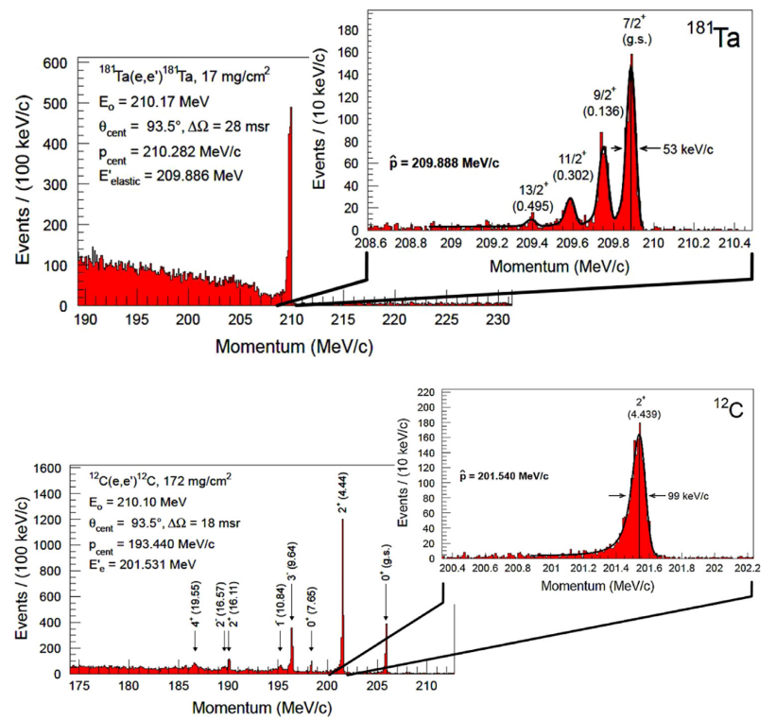
\includegraphics[width=10cm]{image/1-elastic.png}
  \caption[電子弾性散乱によるスペクトロメータ較正]{電子弾性散乱によるスペクトロメータ較正実験で得られる散乱電子スペクトル。210 MeVで$^{181}\text{Ta}$標的と$^{12}\text{C}$標的を用いて電子弾性散乱を行った例を示している。\cite{elastic}}
\end{figure}


しかしこれまでは200 MeV領域の入射電子ビームエネルギー$E_{beam}$の決定精度が$10^{-3}$つまり200 keV程度と大きかった。式(\ref{elastic scattering})からわかるように散乱電子の運動量の決定誤差のオーダーは
$E_{beam}$の決定誤差と同程度であり、結果的に運動量較正の精度も100 keV/c程度になる。
これが100 keV/cの大きな系統誤差の原因である。$10^{-4}$すなわち$20$ keVで電子ビームエネルギーを決定することができれば、崩壊パイ中間子法の実験全体の誤差を統計誤差と同程度の10 keVに抑制することができる。

\section{電子ビームエネルギー測定}
\subsection{MAMIにおける従来手法}
詳細はMAMI加速器の項目で説明する。%
%位置を求めてエネルギーを求めている、そして高エネルギーから外挿するから精度がでない
MAMIで従来使われていた電子ビームエネルギー測定手法は、200 MeV領域の電子ビームエネルギーを直接測定するのではなく、
1.2 GeVの電子ビームエネルギーのビームポジションの測定結果を外挿する形で求められている。
%だから新しい手法が必要
\subsection{逆コンプトン散乱法}
電子ビームエネルギーを直接測定する手法として、逆コンプトン散乱法がある。コンプトン後方散乱法は、電子ビームとレーザー光を衝突させ、
コンプトン散乱で散乱された光子のエネルギーから電子ビームエネルギーを計算する手法である。
レーザー光のエネルギー$E_1$,電子ビームのエネルギーを$\gamma mc^2$,レーザーと電子ビームの衝突角を$\theta$,散乱光子の散乱角を$\phi$として、散乱光子のエネルギー$E_2$は
\begin{eqnarray}
  E_2 = E_1\frac{1+\beta\cos{\theta}}{1-\beta\cos{\phi} + \frac{E_1}{\gamma mc^2} (1-\cos{(\theta +\phi)})} \label{compton}
\end{eqnarray}
と計算できる。電子ビームのエネルギーが高く、レーザー光のエネルギーが十分小さいとして無視できるとき、正面衝突($\theta = 0$)かつ前方散乱($\phi \ll 1$)の場合に散乱光子のエネルギーは最大となり、
\begin{eqnarray}
  E_2 = \frac{4E_1\gamma^2}{1 + \gamma^2\phi^2} \label{compton2}
\end{eqnarray}
と表される。Ge検出器のようなγ線検出器で散乱電子のエネルギーを測定することで、\ref{compton2}式で表される最大エネルギー領域にコンプトンエッジが現れる。このエッジの位置から電子ビームエネルギーを求めることができる。
\begin{figure}
  \centering
  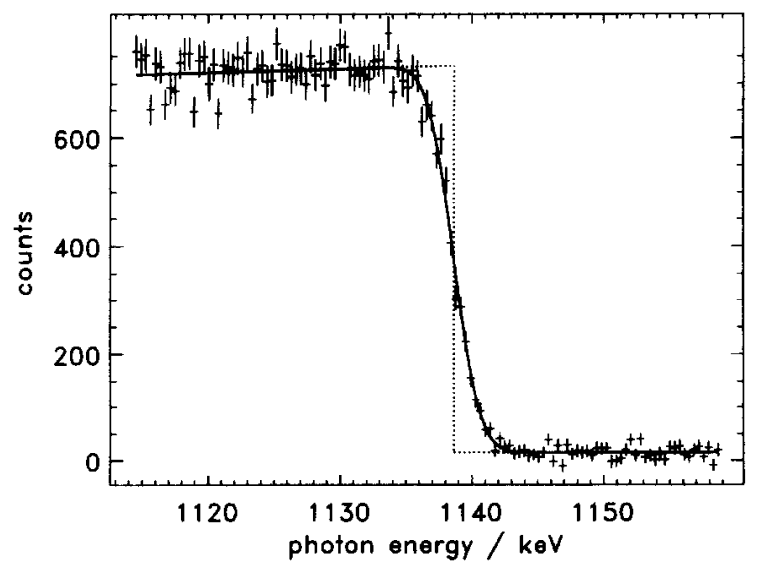
\includegraphics[width=10cm]{image/1-CBS.png}
  \caption[逆コンプトン散乱法]{逆コンプトン散乱法による電子ビームエネルギー測定で得られるコンプトンエッジ\cite{klein1997}}
\end{figure}
しかしながらこの手法で200 MeV領域の電子ビームエネルギーを測定するには、断面積が小さく、高強度の電子ビームが必要となる。%定量的に書く
MAMI加速器では十分な強度の電子ビームを得ることができない。
\subsection{偏極電磁石による電子ビームエネルギー測定}
磁場中を運動する荷電粒子は円運動をする。相対論的運動論によれば、Bの磁場を運動するエネルギー$\gamma mc^2$の電子の運動半径は
\begin{eqnarray}
  r = \frac{\gamma mc}{B}
\end{eqnarray}
である。磁場の精密測定と電子ビームの位置測定によって電子ビームのエネルギーを測定する手法が検討されたが、十分な精度を得ることができなかった。
%定量的に
\subsection{アンジュレータ放射光干渉法の開発の経緯}
崩壊パイ中間子法の系統誤差を抑えるためには、200 MeV領域の電子ビームエネルギーの高精度測定が必要であるが、
従来の手法や既知の手法では十分な精度を得ることができなかった。
そこで我々は2016年からアンジュレータによる放射光を用いた電子ビームエネルギー較正手法(アンジュレータ放射光干渉法)の開発に取り組んできた\cite{klag2018},\cite{klag2023}。
本研究の目的はアンジュレータ放射光干渉法を用いて電子弾性散乱によるスペクトロメータ較正実験を行い、$10^{-4}$以上の電子ビーム絶対値較正精度を達成することである。

%この章のまとめだと思って、200 MeVのエネルギー測定が必要である。そのためにアンジュレータ放射光干渉法を開発している、という話を丁寧にする。
%定量的ゴールを書いておいて、結論でそれを達成したという話をする
\end{document}